%Fiquemos com Deus e Nossa Senhora!
%Sao Jose de Cupertino rogai por nos!!
% ### Uses XeLaTeX ### %
% ### Needs beamer-master ### %
\documentclass[aspectratio=169]{beamer} %. Aspect Ratio 16:9

\usetheme{AI2} % beamerthemeSprace.sty
\usepackage[portuguese]{babel}
\usepackage[utf8]{inputenc}
\usepackage[T1]{fontenc}
\usepackage{ragged2e}

\DeclareMathOperator*{\argmin}{arg\,min}

% DATA FOR FOOTER
\date{2021}
\title{- Regressão Linear}
\author{João Paulo Papa}
\institute{Advanced Institute for Artificial Intelligence (AI2)}

\begin{document}
% ####################################
% FIRST SLIDE 						:: \SliTit{This is the Title of the Talk}{A. B. Name}{Sprace}
% SUB-TITLE SLIDE 					:: \SliSubTit{<title>}{<explanation}
% SUB-SUB-TITLE SLIDE				:: \SliSubSubTit{<title>}{<explanation}
% SLIDE WITH TITLE 					:: \SliT{Title}{Content}
% SLIDE NO TITLE 						:: \Sli{Content} 
% SLIDE DOUBLE COLUMN WITH TITLE 	:: \SliDT{Title}{First Column}{Second Column}
% SLIDE DOUBLE COLUMN NO TITLE 		:: \SliD{First Column}{Second Column}
% SLIDE ADVANCED WITH TITLE 			:: \SliAdvT{Title}{Content}
% SLIDE ADVANCED NO TITLE 			:: \SliAdv{Content}
% SLIDE ADVANCED DOUBLE WITH TITLE 	:: \SliAdvDT{Title}{First Column}{Second Column}
% SLIDE ADVANCED DOUBLE NO TITLE 	:: \SliAdvD{First Column}{Second Column}
% SLIDE BLACK						:: \Black{ <Content> }
% SLIDE WHITE						:: \White{ <Content> }
% ITEMIZATION 						:: \begin{itemize}  \iOn{First} \iTw {Second} \iTh{Third} \end{itemize}
% COMMENT TEXT				 		:: \note{<comment>}
% SECTION 							:: \secx{Section} | \secxx{Sub-Section}
% BOLD SPRACE COLOR				:: \bfs{<text>}
% TABLE OF CONTENT					:: \tocitem{<title>}{<content>}
% LEFT ALIGN EQUATION				:: \begin{flalign*}  & <equation> &   \end{flalign*}
% CENTER ALIGN EQUATION	S			:: \begin{gather*} <equations>  \end{gather*}
% SLASH								:: \slashed{<>}
% BAR								:: \barr{<letter>} instead of \bar{<letter>}
% THEREFORE						:: use \portanto (larger and bold}
% 2 or 3 MATH SYMBOLS				:: \overset{<up>}{<down>} &  \underset{<below>}{\overset{<above>}{<middle>}}  
% INSERT TEXT IN FORMULA			:: \ins{<text>}
% EXERCISE							:: \exe{<exercise #>}{<exercise text>}
% SUGGESTED READING BOX			:: \sug{<references>}
% CITATION							:: \cittex{<citation>}
% CITATION DOUBLE COLUMN 			:: \cittexD{<citation>}
% TEXT POSITION						:: \texpos{<Xcm>}{<Ycm>}{<text>} origin = center of slide : x right | y down
% REFERENCE AT BOTTOM  S/D SLIDE		:: \refbotS{<reference>} \refbotD{<reference>}
% HIDDEN SLIDE						:: \hid
% COLOR BOX 						:: \blu{blue} + \red{rec} + \yel{yellow} + \gre{green} + \bege{beige}
% FRAME 							:: \fra{sprace} \frab{blue} \frar{red} + \fray{yellow} + \frag{green}		
% FIGURE 							:: \img{X}{Y}{<scale>}{Figure.png} 
% FIGURE							:: \includegraphics[scale=<scale>]{Figures/.png}
% FIGURE DOUBLE SLIDE NO TITLE		::  \img{-4}{0.5}{<scale>}{Figure.png} % Image 1st half
%									::  \img{4}{0.5}{<scale>}{Figure.png} % Image 2nd half
% FIGURE DOUBLE SLIDE WITH TITLE		::  \img{-4}{0}{<scale>}{Figure.png} % Image 1st half
%									::  \img{4}{0}{<scale>}{Figure.png} % Image 2nd half
% INCLUDING SWF (Flash)				:: \usepackage{media9} and \includemedia >> USE ACROBAT <<
%%%%%%%%%%%%%%%%%%%%%%%%%%%%%%%%%%%%%%%%%%%%%%%%%%
% ###############################################################################
% FIRST SLIDE
\SliTit{Regressão Linear}{Advanced Institute for Artificial Intelligence -- AI2}{https://advancedinstitute.ai}
%%%%%%%%%%%%%%%%%%%%%%%%%%%%%%%%%%%%%%%%%%%%%%%%%%
% ###############################################################################
% SLIDE SUB-TITLE
%\SliSubTit{Sub-Title}{Description}{}
%%%%%%%%%%%%%%%%%%%%%%%%%%%%%%%%%%%%%%%%%%%%%%%%%%
% ###############################################################################
%\SliSubSubTit{Sub-Sub-Title}{Description}
 %%%%%%%%%%%%%%%%%%%%%%%%%%%%%%%%%%%%%%%%%%%%%%%%%%


\SliT{Introdução}{
\secx{Regressão Linear Univariada}

\justifying Em aprendizado de máquina, existem diversos problemas para os quais conhecemos um conjunto de valores de entrada e desejamos \textbf{estimar} o valor de saída. Um exemplo bastante comum é a precificação de imóveis, cujo valor de entrada corresponde ao tamanho de uma casa e a saída desejada é o seu preço.

\begin{center}
\onslide<2->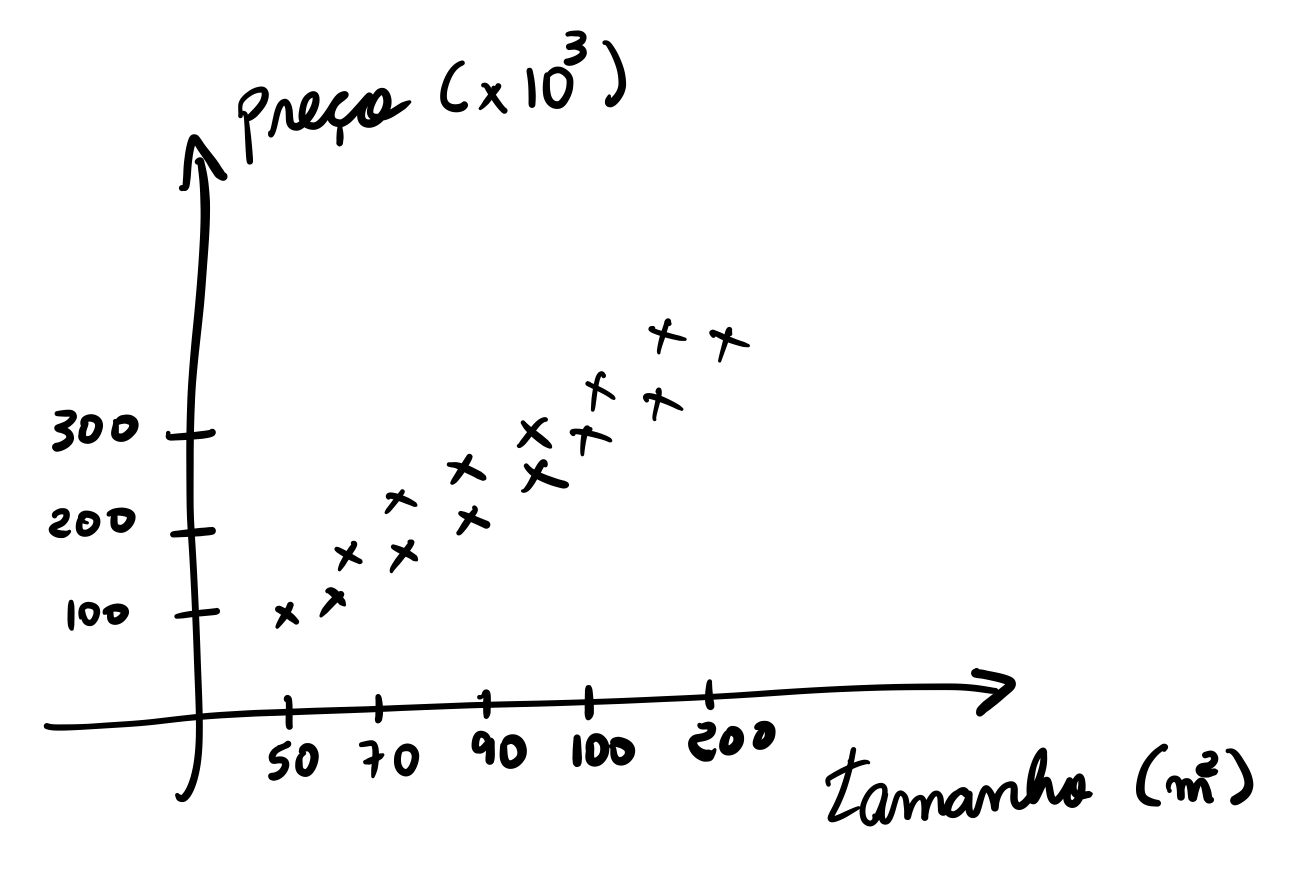
\includegraphics[scale=0.1]{./figs/Regressao_Linear_Fig1.png}
\onslide<3->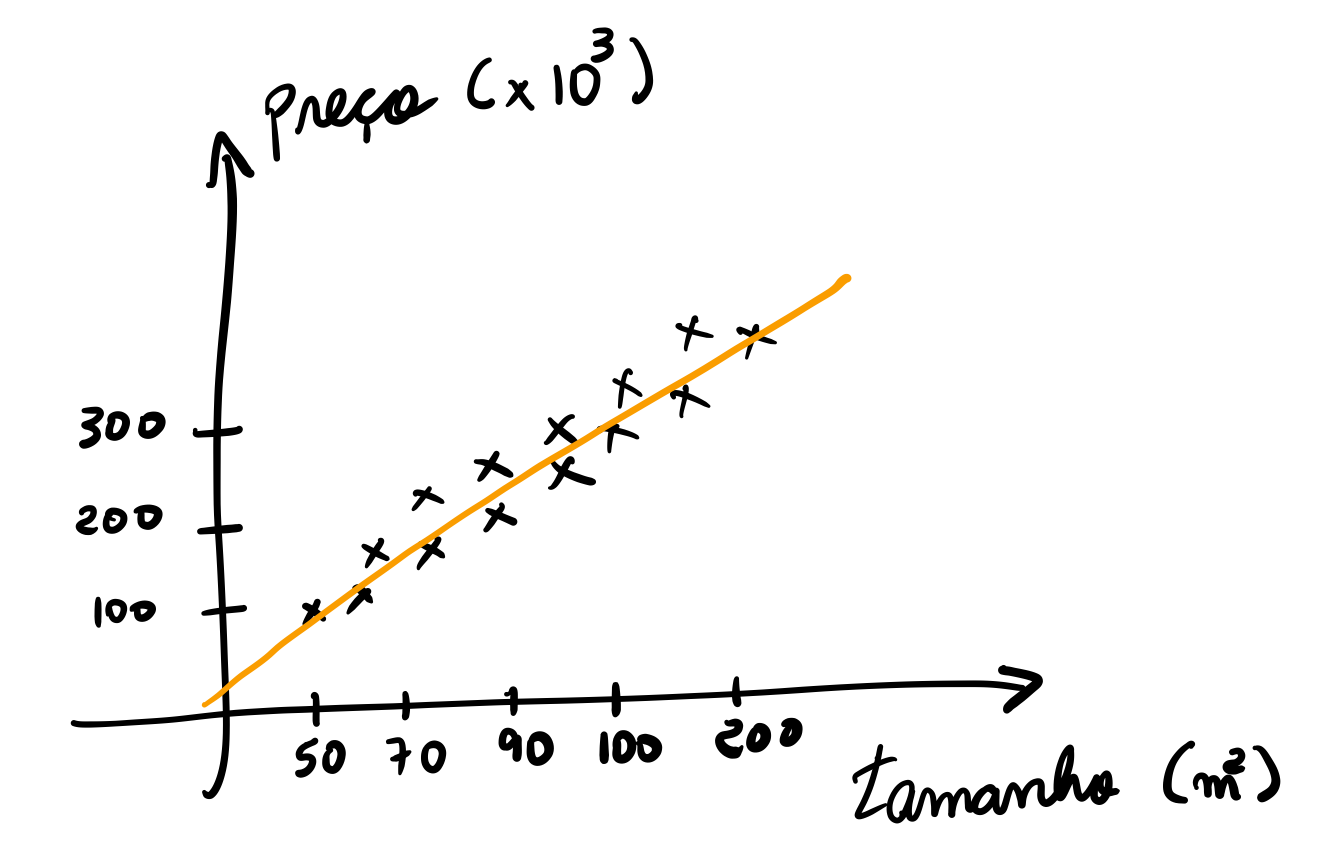
\includegraphics[scale=0.1]{./figs/Regressao_Linear_Fig2.png}
\end{center}

%\secxx{Sub-Section}

% EXERCISE
%\exe{4}{Exercise}
% SUGGESTED READING BOX			
%\sug{References}
% CITATION						
%\cittex{Citation}

}%%%%%%%%%%%%%%%%%%%%%%%%%%%%%%%%%%%%%%%%%%%%%%%%%%
% ###############################################################################
% SLIDE NO TITLE
\Sli{
\justify \underline{Definição do problema:} seja um conjunto de dados ${\cal X}= \{(x_1,y_1),(x_2,y_2),\ldots,(x_z,y_z)\}$ tal que $x_i\in\mathbb{R}$ corresponde ao dado de entrada e $y_i\in\mathbb{R}$ denota o seu respectivo valor de saída. Temos, ainda, que ${\cal X}$ pode ser \textbf{particionado} da seguinte forma: ${\cal X} = {\cal X}^1\cup {\cal X}^2$, em que ${\cal X}^1$ e ${\cal X}^2$ denotam os conjuntos de dados de \textbf{treinamento} e \textbf{teste}, respectivamente. Nosso objetivo é, dado o conjunto de treinamento, aprender uma função $h:\mathbb{R}\rightarrow\mathbb{R}$ que consiga estimar o valor de uma casa dado o seu tamanho.

\begin{center}
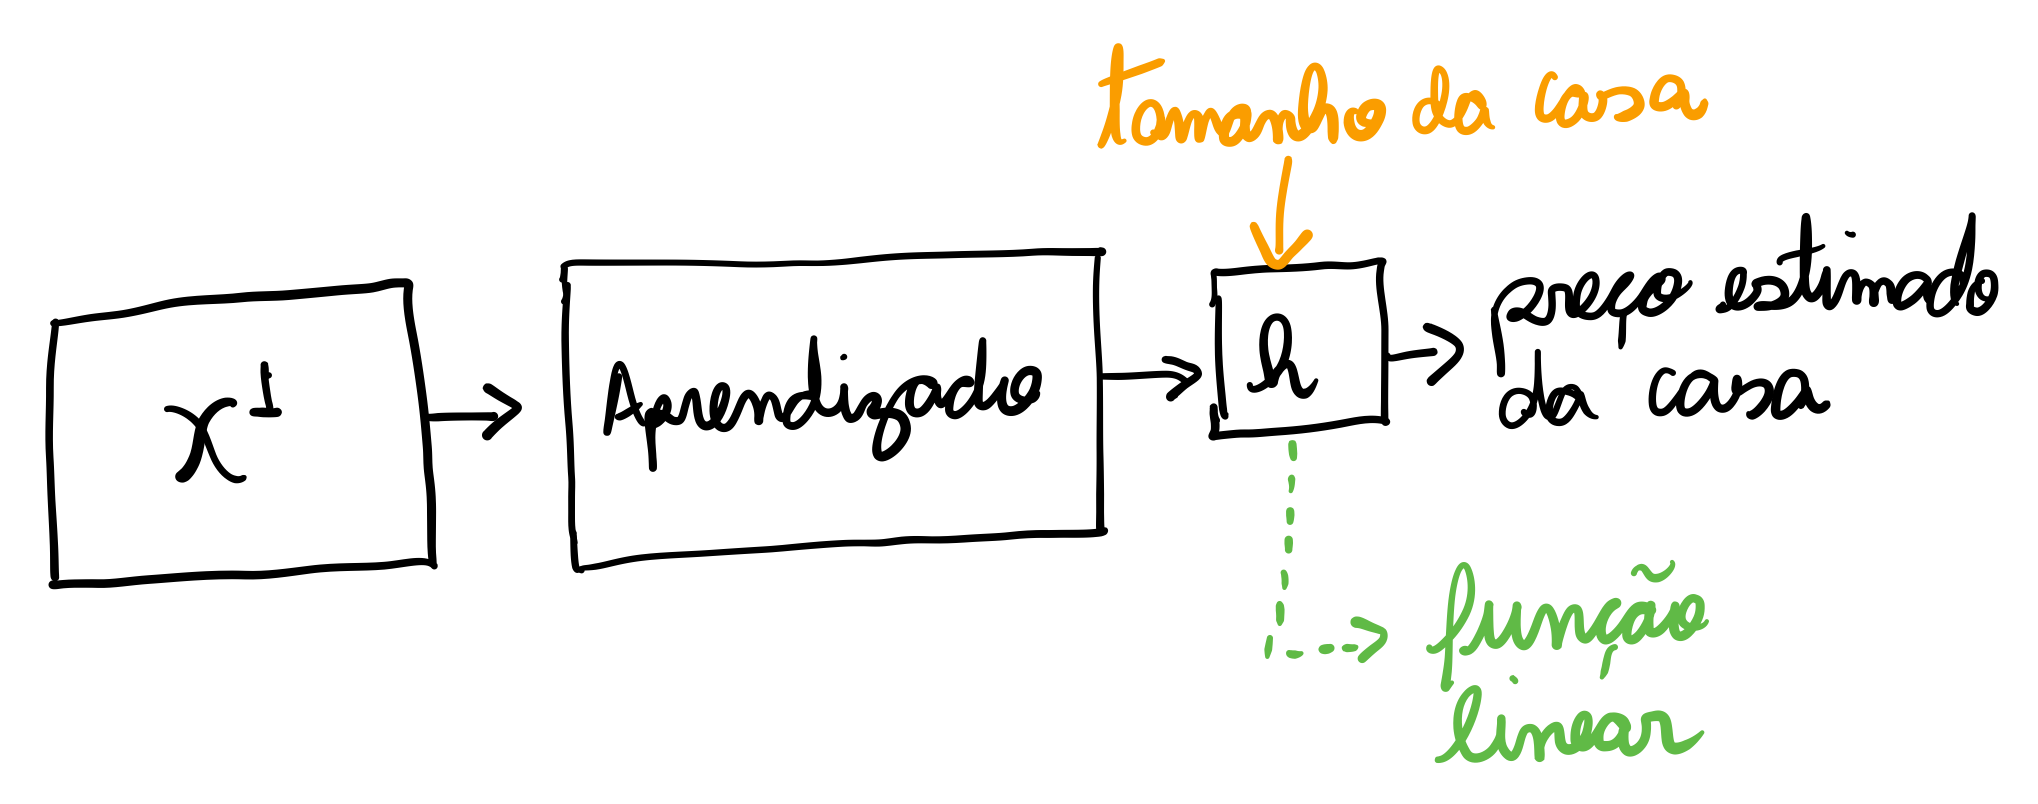
\includegraphics[scale=0.1]{./figs/Regressao_Linear_Fig3.png}
\end{center}
}

\Sli{
\justify A técnica chama-se \textbf{Regressão Linear Univariada} porque aprendemos uma \textbf{função linear} utilizando apenas \textbf{uma} variável de entrada. Desta forma, temos a seguinte formulação para essa função:

\begin{equation}
\label{e.hx}
	h_{\boldsymbol{w}}(x)=w_0+w_1x,
\end{equation}
em que $w_0$ e $w_1$ denotam os parâmetros do modelo (equação da reta), podendo ser representados como $\boldsymbol{w}=[w_0\ w_1]$.

\begin{center}
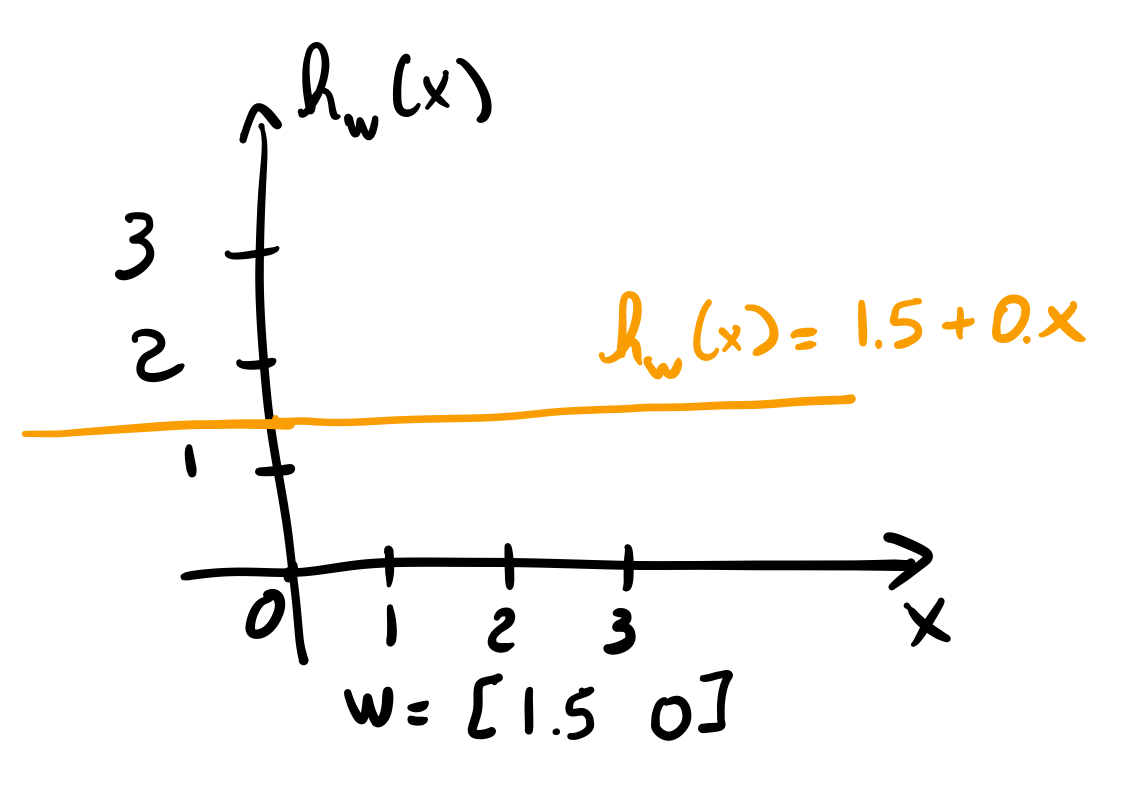
\includegraphics[scale=0.1]{./figs/Regressao_Linear_Fig4.png}\hspace{1cm}
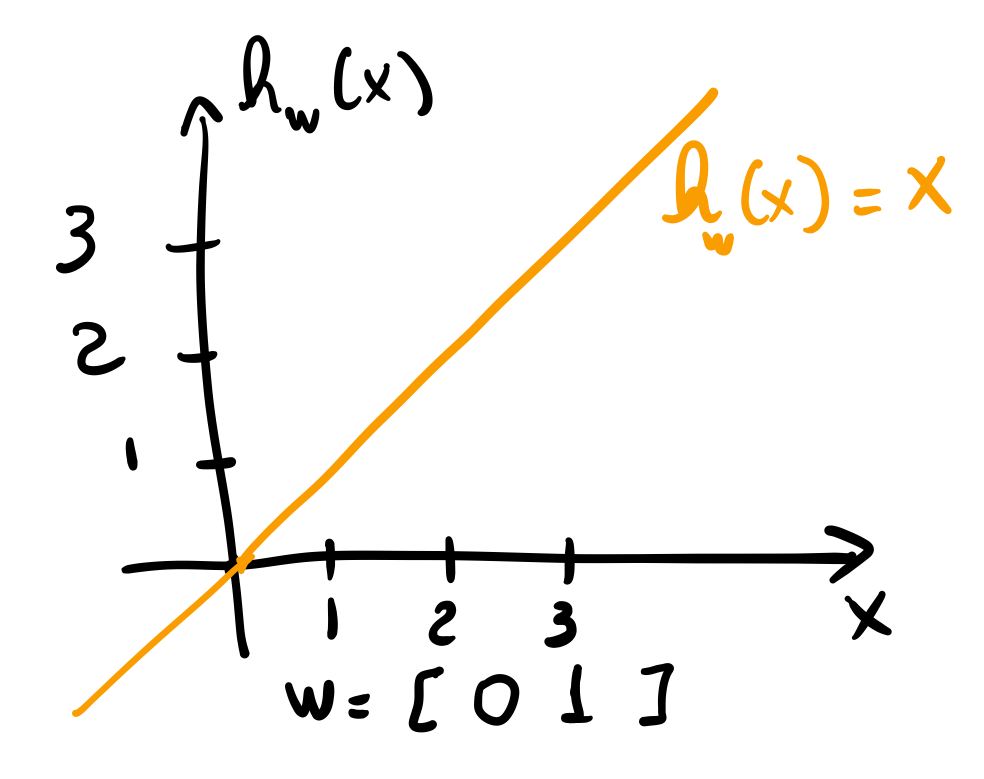
\includegraphics[scale=0.1]{./figs/Regressao_Linear_Fig5.png}\hspace{1cm}
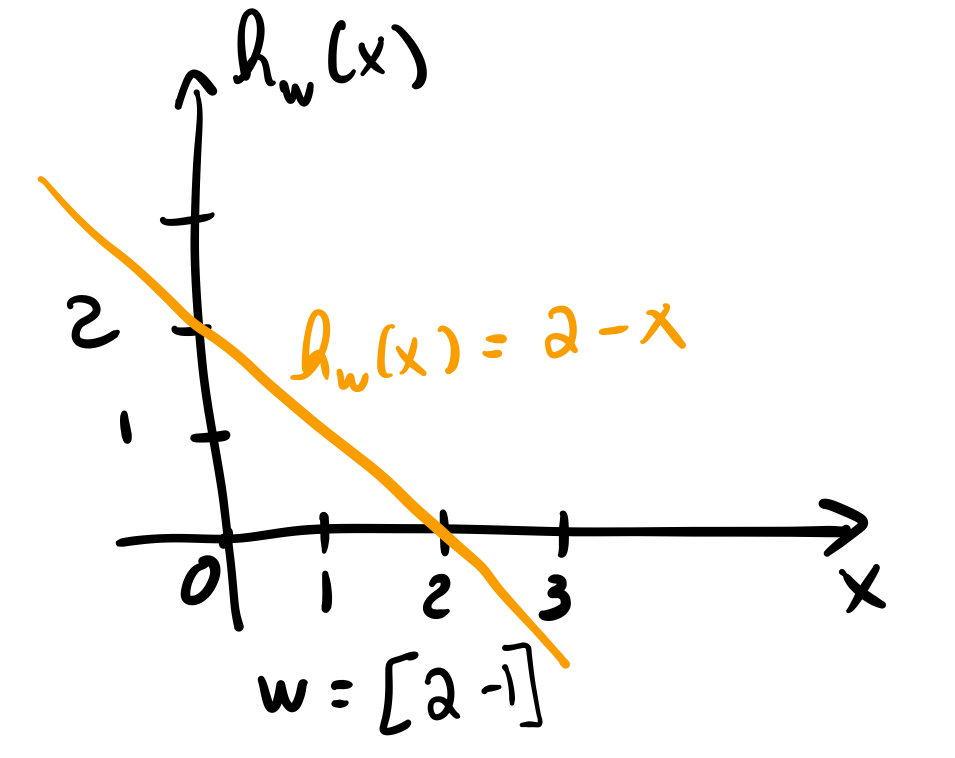
\includegraphics[scale=0.1]{./figs/Regressao_Linear_Fig6.png}
\end{center}

}%%%%%%%%%%%%%%%%%%%%%%%%%%%%%%%%%%%%%%%%%%%%%%%%%%

\Sli{
\justify Desta forma, como podemos observar, temos diferentes comportamentos para $h_{\boldsymbol{w}}(x)$, a qual é também chamada de \textbf{função hipótese}. A ideia principal da regressão linear é escolher o vetor de parâmetros $\boldsymbol{w}$ tal que $h_{\boldsymbol{w}}(x)$ seja a mais próxima possível das saídas das amostras de nosso conjunto de treinamento. Matematicamente falando, temos o seguinte problema de \textbf{minimização}:

\begin{equation}
\label{e.min_linear_regression}
	\boldsymbol{w}^\ast = \argmin_{\boldsymbol{w}}\left\{\frac{1}{2m}\sum_{i=1}^m(h_w(x_i)-y_i)^2\right\},
\end{equation}
em que $m$ denota o tamanho do conjunto de treinamento. Essa formulação corresponde ao conhecido \textbf{erro médio quadrático}, do inglês \emph{mean squared error} (MSE).
}

\Sli{
A Equação 2 é usualmente chamada de \textbf{função de custo} ou \textbf{função de perda}, também conhecida por \textbf{erro médio quadrático}. Podemos simplificar a notação escrevendo a Equação 2 da seguinte forma:

\begin{equation}
\label{e.min_linear_regression_simplified}
	\boldsymbol{w}^\ast = \argmin_{\boldsymbol{w}}\{J(\boldsymbol{w})\},
\end{equation}
em que 

\begin{equation}
\label{e.cost_function}
J(\boldsymbol{w}) = \frac{1}{2m}\sum_{i=1}^m(h_w(x_i)-y_i)^2. 
\end{equation}
No entanto, vamos simplificar um pouco mais o problema e assumir que $\boldsymbol{w} = [0\ w_1]$, ou seja, vamos assumir que $w_0 = 0$ (a reta passa na origem do sistema de coordenadas).
}

\Sli{
Assim sendo, a Equação 1 pode ser escrita da seguinte forma:

\begin{equation}
	h_{\boldsymbol{w}}(x)  = w_0 +w_1x = w_1x.
\end{equation}

\begin{center}
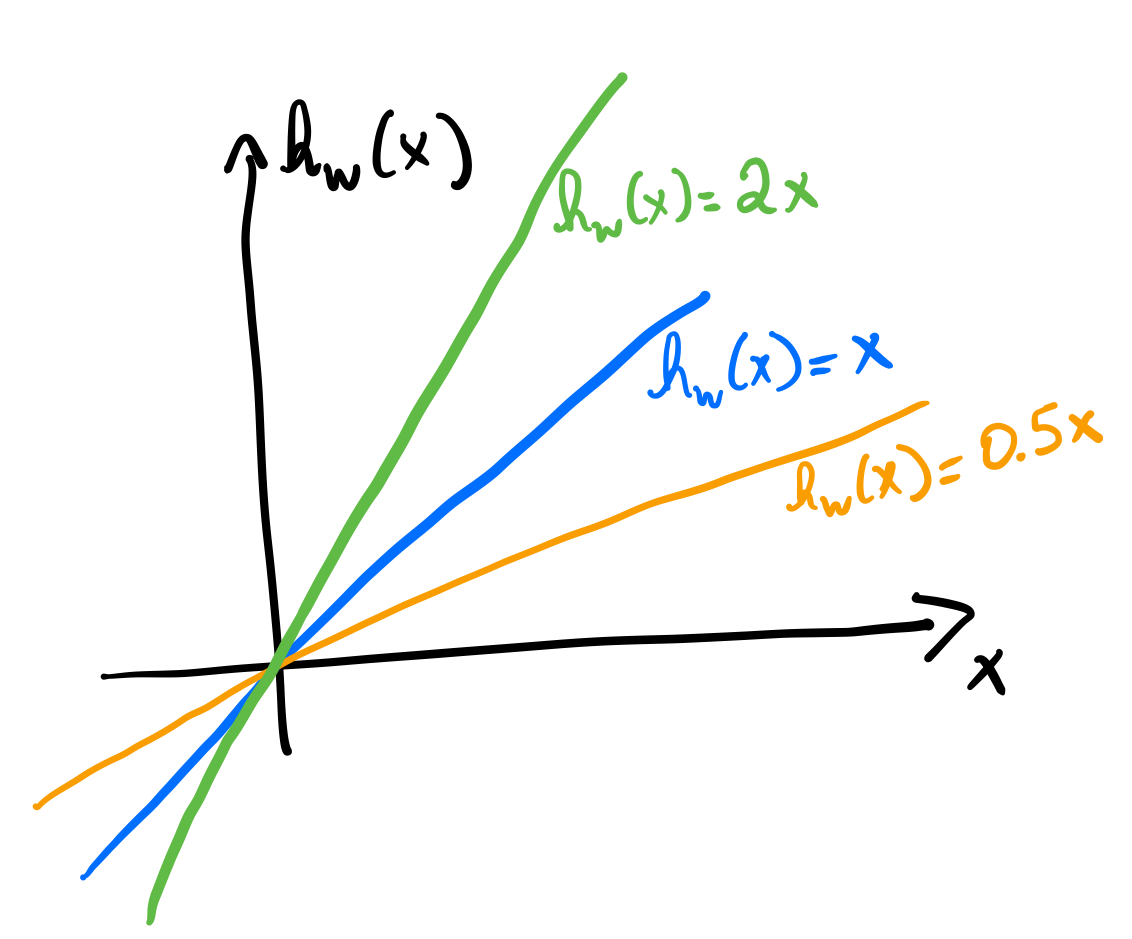
\includegraphics[scale=0.13]{./figs/Regressao_Linear_Fig7.png}\hspace{1cm}
\end{center}
}

\Sli{
Assumindo, então, que $w_0=0$, podemos escrever a Equação 3 da seguinte forma:

\begin{equation}
\label{e.min_linear_regression_simplified}
	\boldsymbol{w}^\ast = \argmin_{w_1}\left\{J(w_1)\right\}.
\end{equation}
\justify O nosso problema passar a ser, agora, encontrar um valor apropriado para $w_1$ de tal forma que o valor de $J(w_1)$ seja o menor possível. Resumindo, o que temos definido até então para o problema:

\begin{itemize}
	\item Função hipótese: $h_{\boldsymbol{w}}(x)\approx w_1x$
	\item Função de custo: $J(\boldsymbol{w})\approx J(w_1)$
\end{itemize}
}

\Sli{
Vamos ilustrar algumas situações para entendermos o comportamento de ambas funções (hipótese e custo). Suponha o conjunto de treinamento ${\cal X}^1=\{(1,1),(2,2),(3,3)\}$. Neste caso, temos que $m=3$. Ademais, suponha que $h_{\boldsymbol{w}}(x) = x$, ou seja, $w_1=1$.

\begin{minipage}{0.3\textwidth}
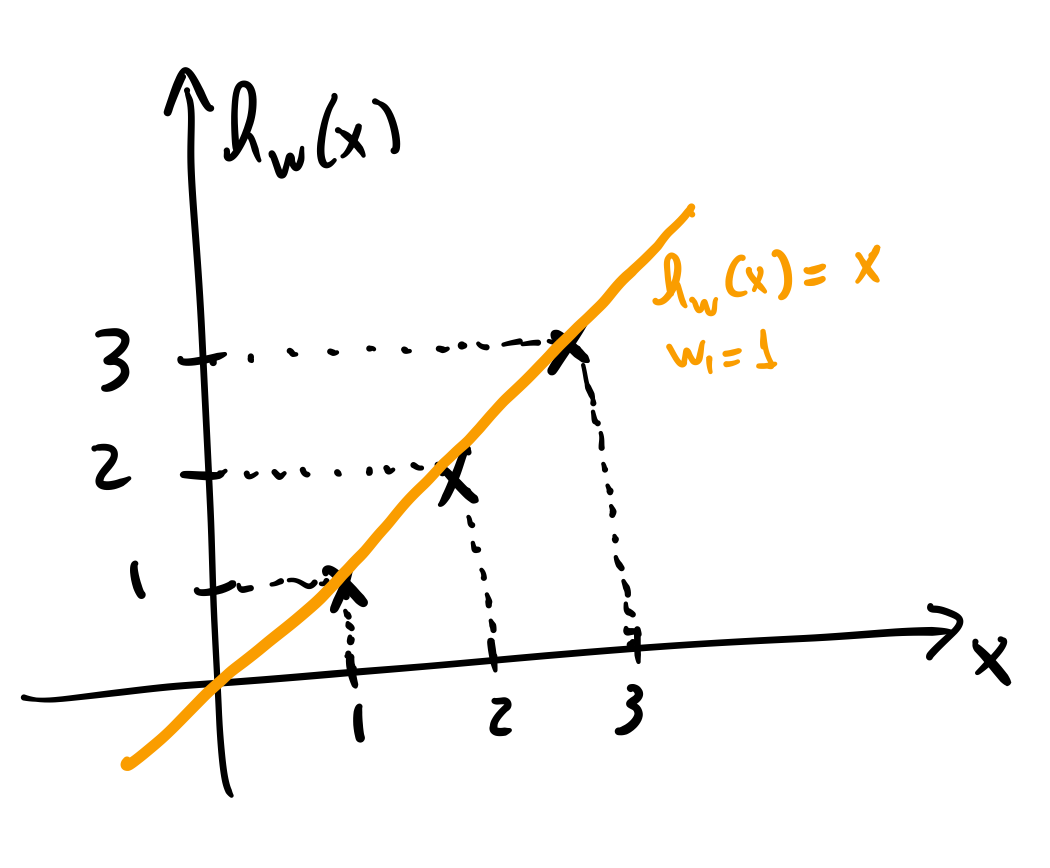
\includegraphics[scale=0.13]{./figs/Regressao_Linear_Fig8.png}
\end{minipage}%%% to prevent a space
\begin{minipage}{0.37\textwidth}
\scriptsize
\begin{equation}\nonumber
\begin{split}
J(w_1) &= \frac{1}{2m}\sum_{i=1}^3(h_{\boldsymbol{w}}(x_i)-y_i)^2\\
&= \frac{1}{2m}\sum_{i=1}^3(w_1x_i-y_i)^2\\
&= \frac{1}{2m}\sum_{i=1}^3(x_i-y_i)^2\\
&= \frac{1}{2.3}[(1-1)^2+(2-2)^2+(3-3)^2]\\
&= 0
\end{split}
\end{equation}
\null
\par\xdef\tpd{\the\prevdepth}
\end{minipage}
\begin{minipage}{0.3\textwidth}
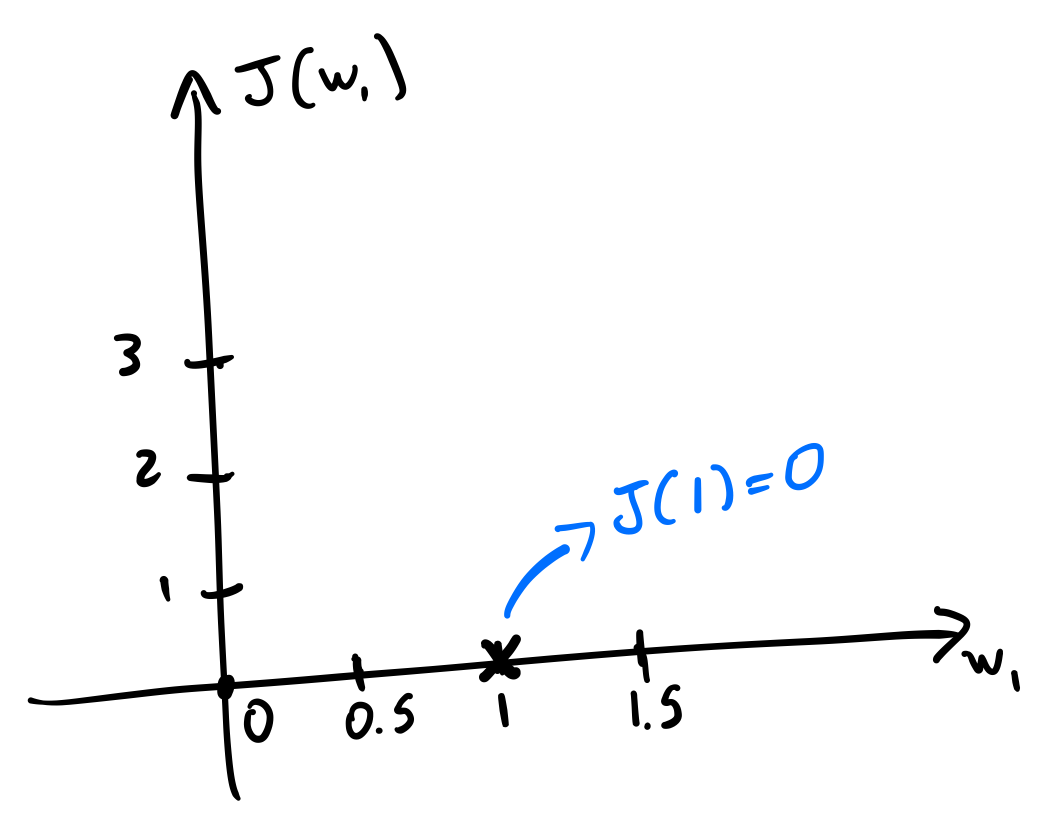
\includegraphics[scale=0.13]{./figs/Regressao_Linear_Fig9.png}
\end{minipage}%%% to prevent a space
}	

\Sli{
Agora, suponha que a nossa função hipótese é dada por $h_{\boldsymbol{w}}(x) = 0.5x$, ou seja, $w_1 = 0.5$.

\begin{minipage}{0.27\textwidth}
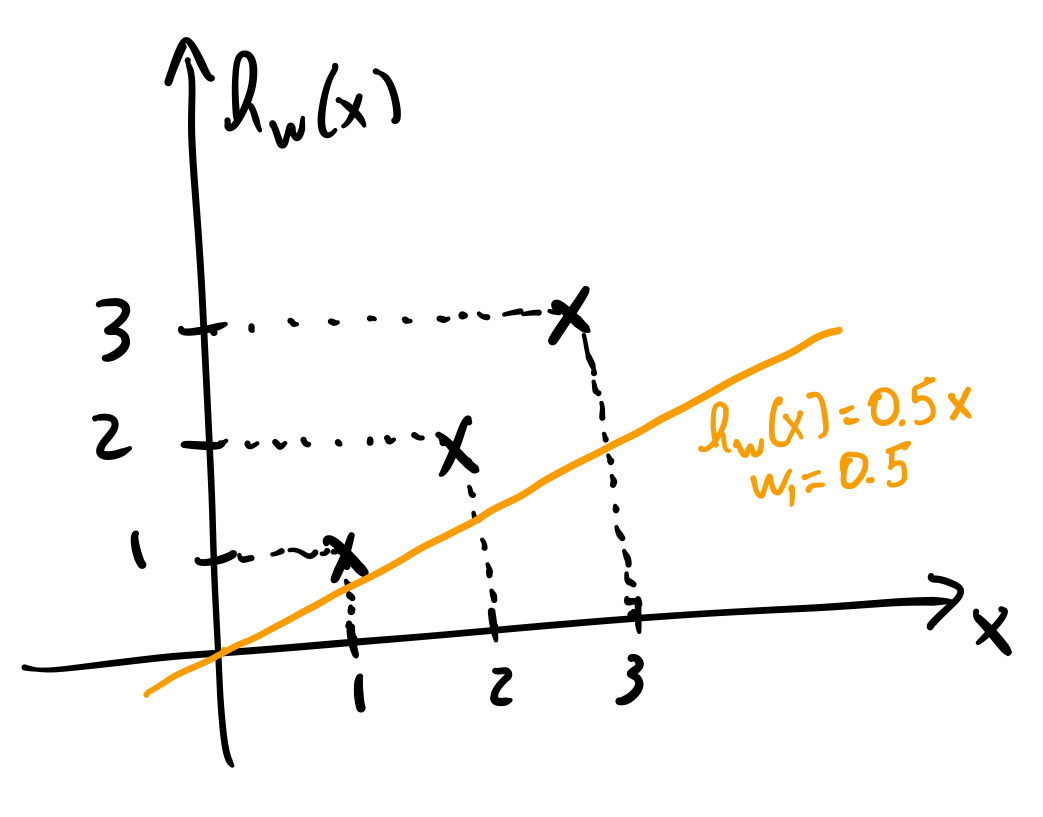
\includegraphics[scale=0.11]{./figs/Regressao_Linear_Fig10.png}
\end{minipage}%%% to prevent a space
\begin{minipage}{0.4\textwidth}
\scriptsize
\begin{equation}\nonumber
\begin{split}
J(w_1) &= \frac{1}{2.3}[(0.5-1)^2+(1-2)^2+(1.5-3)^2]\\
&= \frac{1}{2.3}(0.25+1+2.25)\\
&= \frac{1}{6}(3.5)\\
&\approx 0.58
\end{split}
\end{equation}
\null
\par\xdef\tpd{\the\prevdepth}
\end{minipage}
\begin{minipage}{0.27\textwidth}
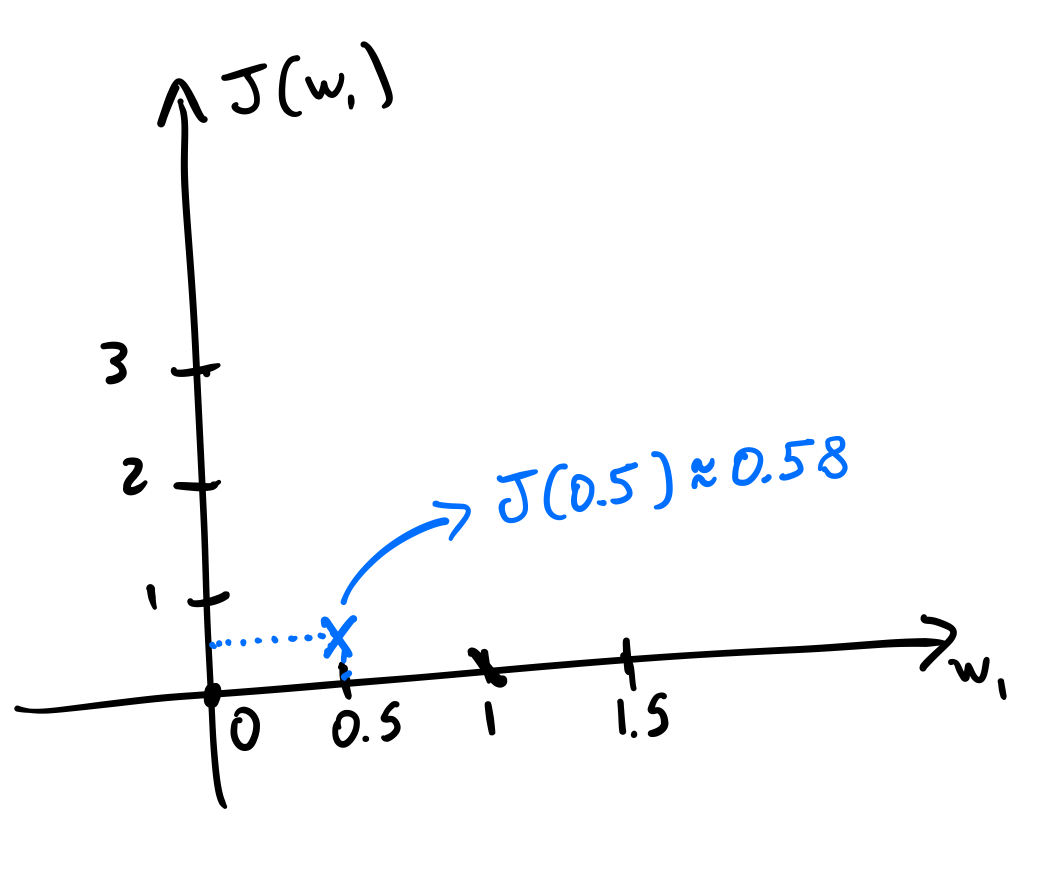
\includegraphics[scale=0.11]{./figs/Regressao_Linear_Fig11.png}
\end{minipage}%%% to prevent a space
}

\Sli{
Qual o comportamento da função de custo caso tenhamos diferentes valores para $w_1$?

\begin{center}
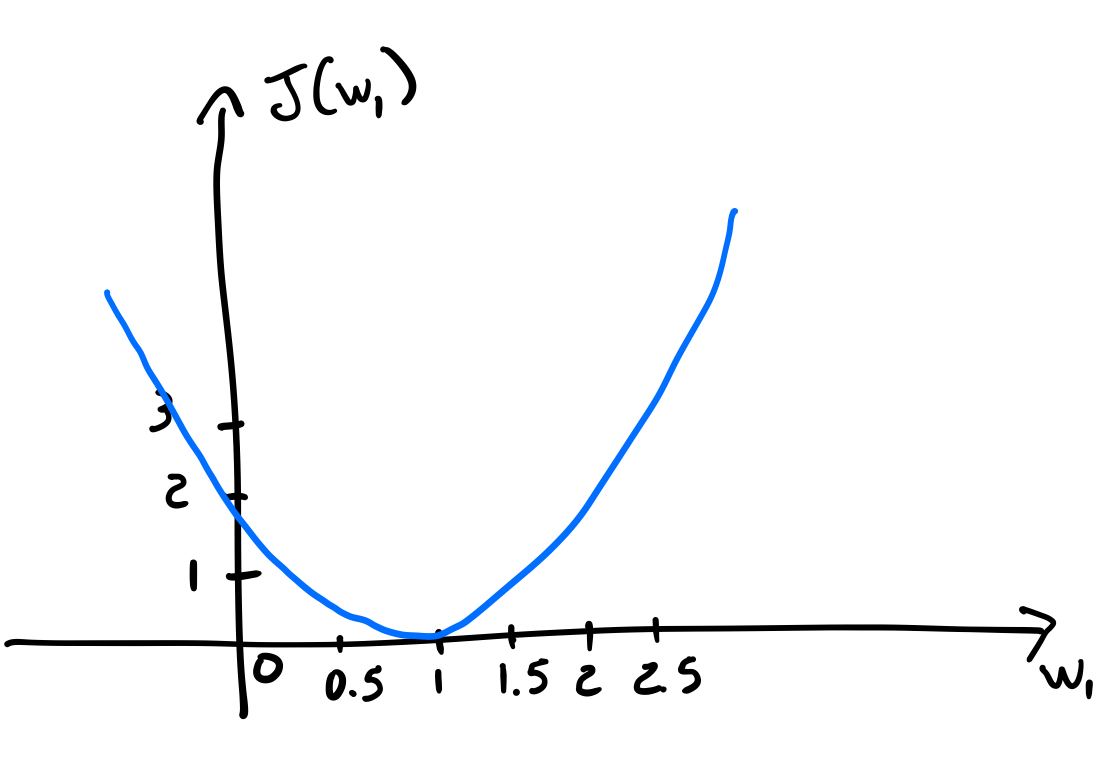
\includegraphics[scale=0.17]{./figs/Regressao_Linear_Fig12.png}
\end{center}

Desta forma, temos que $\boldsymbol{w}^\ast = w_1 = 1$ é o valor \textbf{ótimo}, ou seja, aquele que minimiza o valor de $J(w_1)$. 
}

\Sli{
\justify Uma alternativa ao uso do MSE é o chamado \textbf{erro médio absoluto}, do inglês \emph{mean absolute error} (MAE). Mas qual o intuito de utilizarmos MSE? Notem que o formato da função de custo nos remete à uma função quadrática!

\justify A pergunta agora é: como podemos escolher bons valores para $\boldsymbol{w} = [w_0\ w_1]$? Podemos usar o método da \textbf{força bruta} testando um número suficientemente grande valores de aleatórios para $\boldsymbol{w}$. É uma boa abordagem?

}

\Sli{
\justify Uma solução é o uso da técnica conhecida por \textbf{gradiente descendente}, que faz a busca pelos valores de $\boldsymbol{w}$ baseando-se na \textbf{derivada} da função de custo. Como ele funciona?

\begin{enumerate}
	\item Atribua valores aleatórios para $\boldsymbol{w} = [w_0\ w_1]$.
	\item Avalie a função de custo $J(\boldsymbol{w})$.
	\item  Caso o \textbf{critério de parada tenha sido atingido}, vá para o passo 5.
	\item Atualize o vetor $\boldsymbol{w}$ e retorne ao Passo 2.
	\item Fim do algoritmo.
\end{enumerate}
}

\Sli{
\justify Qual o problema? As funções de custo geralmente não são \textbf{convexas}.

\begin{center}
\begin{tabular}{cc}
\hspace{0.7cm}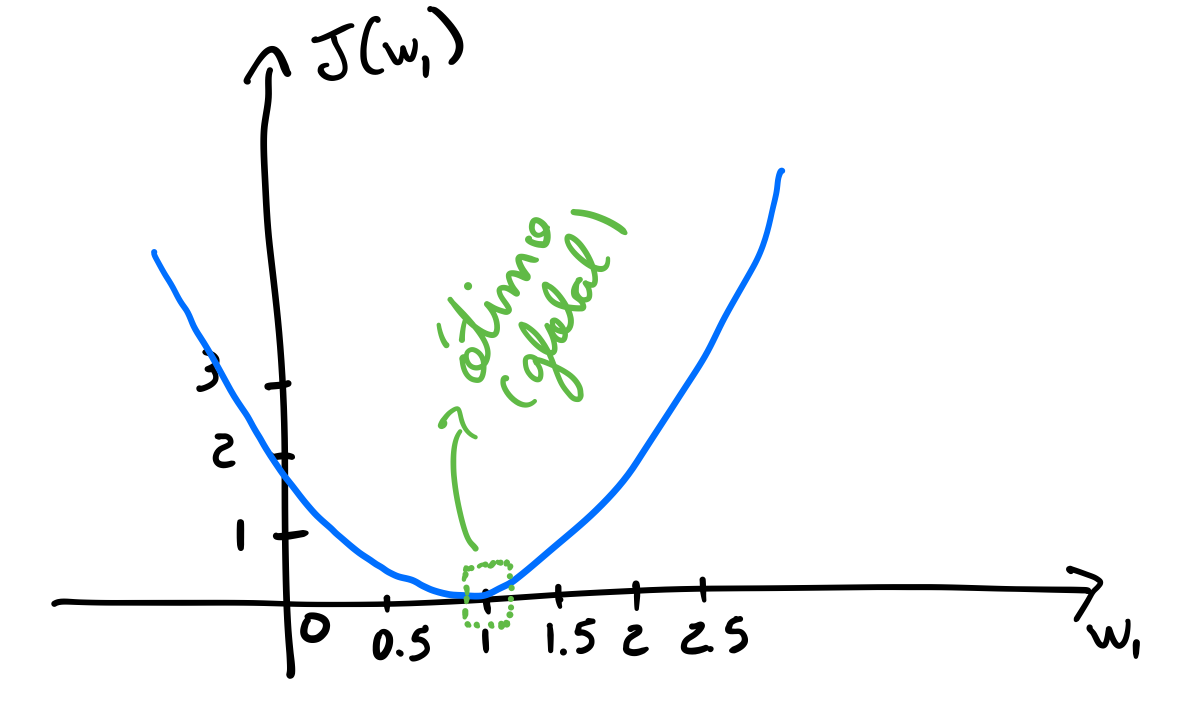
\includegraphics[scale=0.13]{./figs/Regressao_Linear_Fig13.png}\hspace{1cm} &
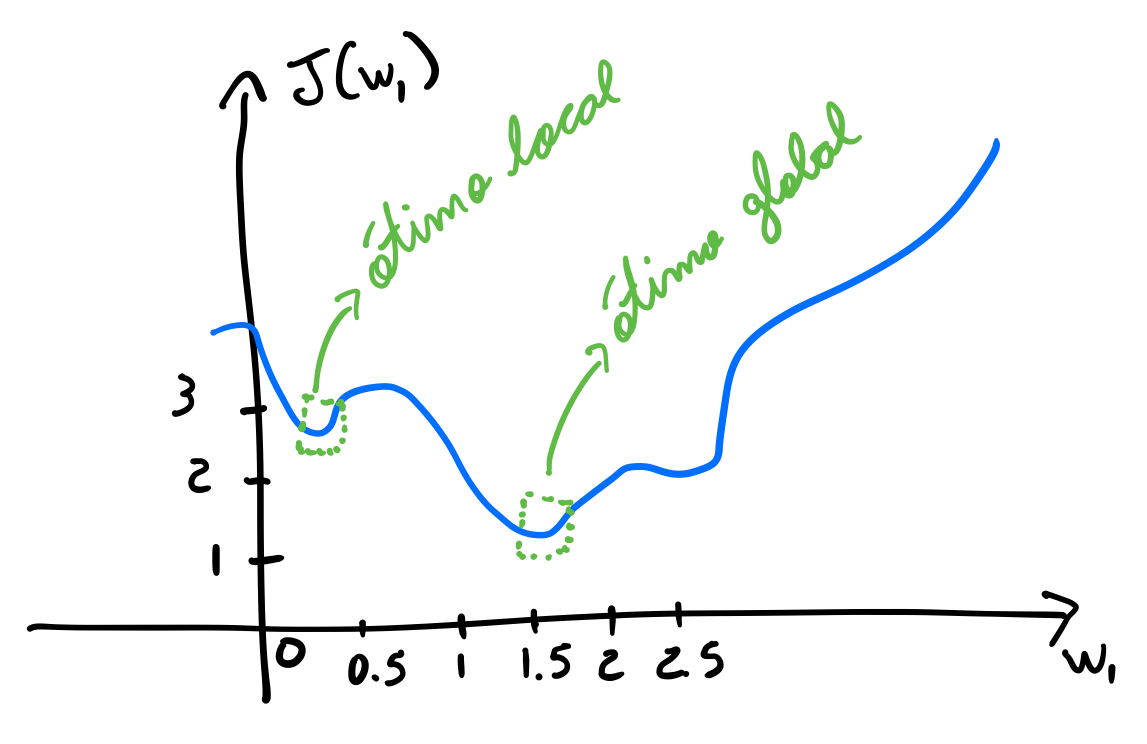
\includegraphics[scale=0.13]{./figs/Regressao_Linear_Fig14.png}\hspace{1cm}\\
Função convexa & Função não convexa
\end{tabular}
\end{center}
}

\Sli{
\justify Gradiente descendente busca a ``melhor"\ solução a partir de um ponto inicial. Com base em informações dadas pela \textbf{derivada} da função, ele tende a encontrar um ótimo local ou global. Caso a função seja convexa, ele encontrará o ótimo global. Quais as informações que a derivada nos dá?

\begin{center}
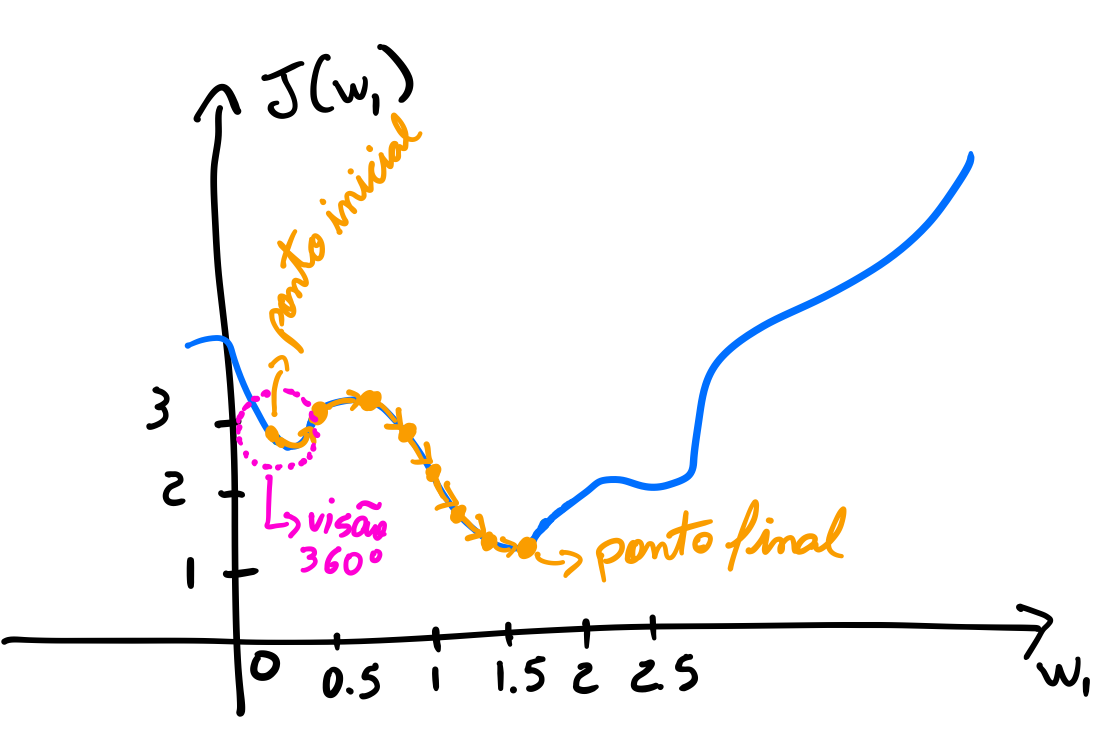
\includegraphics[scale=0.157]{./figs/Regressao_Linear_Fig15.png}\hspace{1cm}
\end{center}
}

\Sli{
Matematicamente falando, podemos modelar a ideia por meio da \textbf{regra de atualização} dos parâmetros de $\boldsymbol{w}$:

\begin{equation}
	w_j^{(t+1)} = w_j^{(t)}-\alpha\frac{\partial J(\boldsymbol{w})}{\partial w_j},
\end{equation}
em que $j\in\{0,1\}$ e $\alpha$ corresponde à \textbf{taxa de aprendizado}. Já o termo $\frac{\partial J(\boldsymbol{w})}{\partial w_j}$ denota a \textbf{derivada parcial}, que deverá ser calculada para cada parâmetro de nossa equação da reta.
}

\Sli{
\justify A questão principal que temos agora é: como calcular o termo derivativo, ou seja, as derivadas parciais? Para fins de simplicidade, suponha, novamente que $w_0 = 0$. Assim, nosso objetivo passa a ser o de minimizar $J(w_1)$ para algum valor $w_1\in\mathbb{R}$.

\begin{center}
\begin{minipage}{0.37\textwidth}
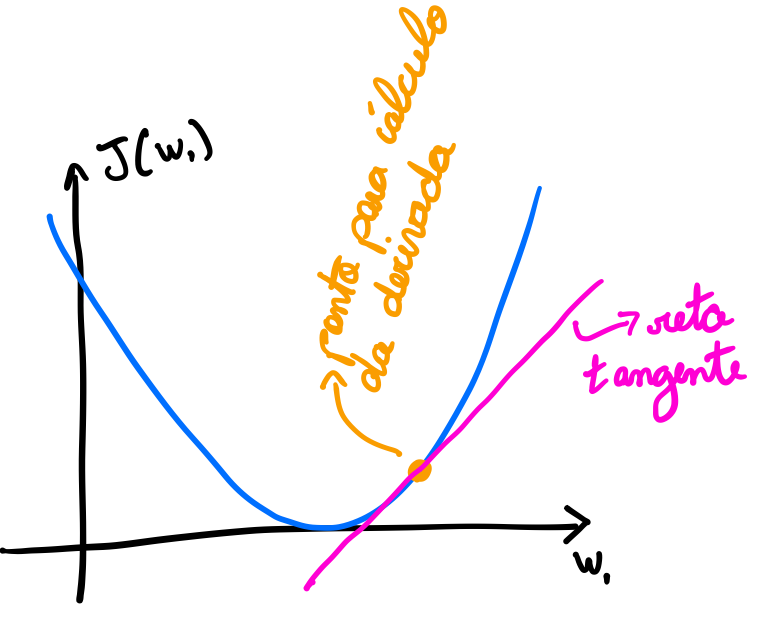
\includegraphics[scale=0.157]{./figs/Regressao_Linear_Fig16.png}
\end{minipage}%%% to prevent a space
\begin{minipage}{0.37\textwidth}
A derivada em um ponto nos retorna duas principais informações: \textbf{direção} e \textbf{magnitude}. A primeira é dada pela inclinação (sinal) da reta tangente no ponto que desejamos calcular a derivada.
\null
\par\xdef\tpd{\the\prevdepth}
\end{minipage}
\end{center}

Neste exemplo, a inclinação é positiva, ou seja, $\frac{\partial J(\boldsymbol{w})}{\partial w_j}>0$. Desta forma, estamos diminuindo o valor de $w_1$.
}

\Sli{
Já no exemplo abaixo, temos que a inclinação da reta é negativa, ou seja, $\frac{\partial J(\boldsymbol{w})}{\partial w_j}<0$. Assim, estamos aumentando o valor de $w_1$.

\begin{center}
	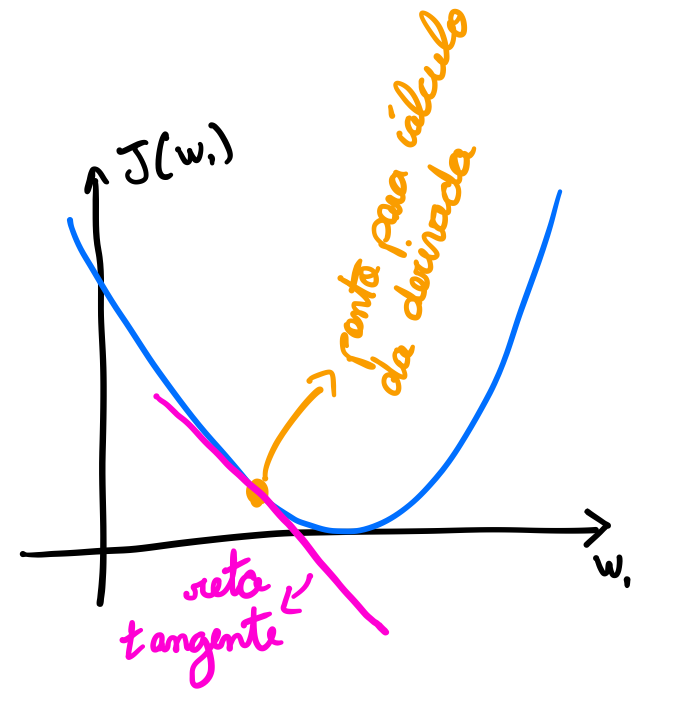
\includegraphics[scale=0.17]{./figs/Regressao_Linear_Fig17.png}
\end{center}

A informação de magnitude é o próprio valor retornado pelo termo derivativo, desconsiderando o sinal.
}

\Sli{
Qual a importância da taxa de aprendizado na Equação 7? Basicamente, baixos valores de $\alpha$ nos levam à uma convergência mais lenta, ao passo que valores maiores podem acelerar esse processo. No entanto, precisamos tomar cuidado com essa escolha.

\begin{tabular}{ccc}
	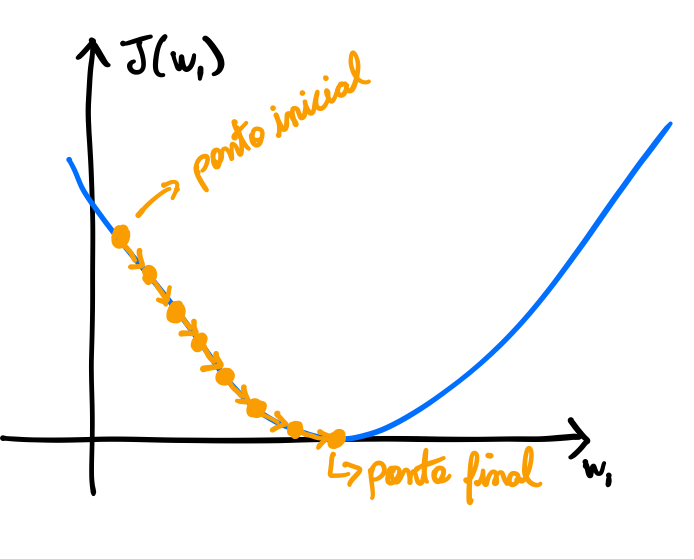
\includegraphics[scale=0.17]{./figs/Regressao_Linear_Fig18.png} &
	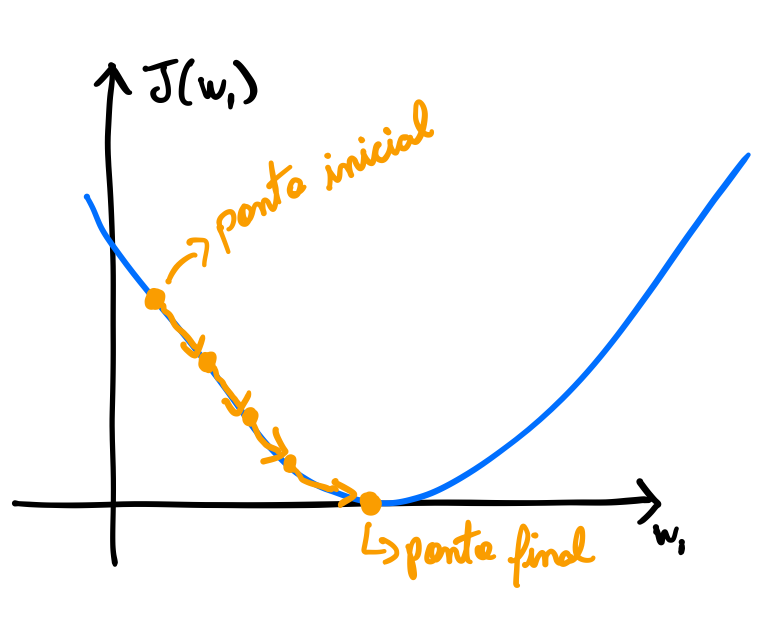
\includegraphics[scale=0.17]{./figs/Regressao_Linear_Fig19.png} &
	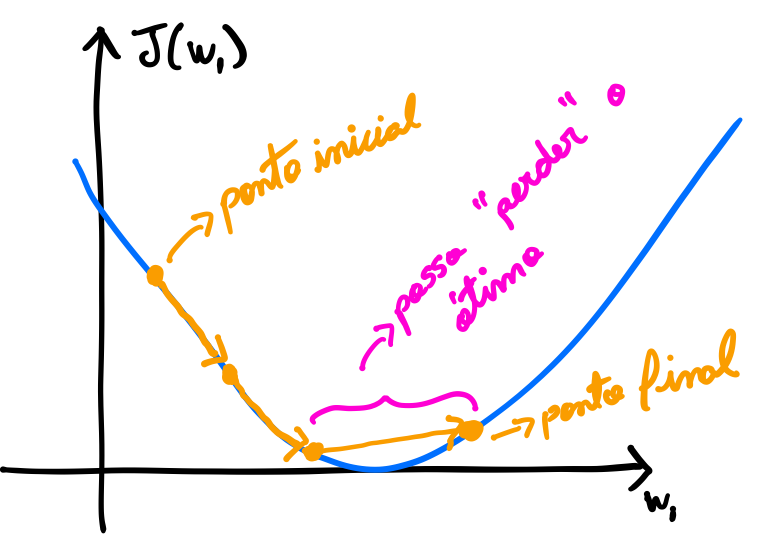
\includegraphics[scale=0.17]{./figs/Regressao_Linear_Fig20.png} \\
	(a) $\alpha$ pequeno & (b) $\alpha$ adequado & (c) $\alpha$ grande
\end{tabular}
}

\Sli{
No entanto, o que acontece com o gradiente descendente se a inicialização ocorrer em um ótimo local? A inclinação é igual à 0!

\begin{minipage}{0.37\textwidth}
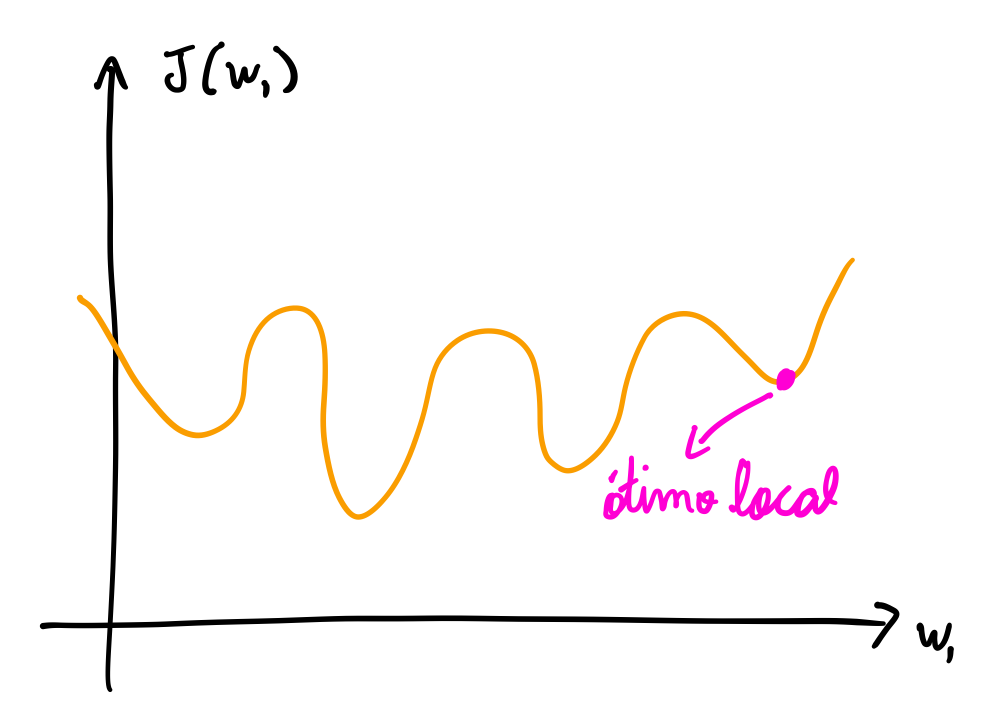
\includegraphics[scale=0.157]{./figs/Regressao_Linear_Fig21.png}
\end{minipage}%%% to prevent a space
\begin{minipage}{0.27\textwidth}
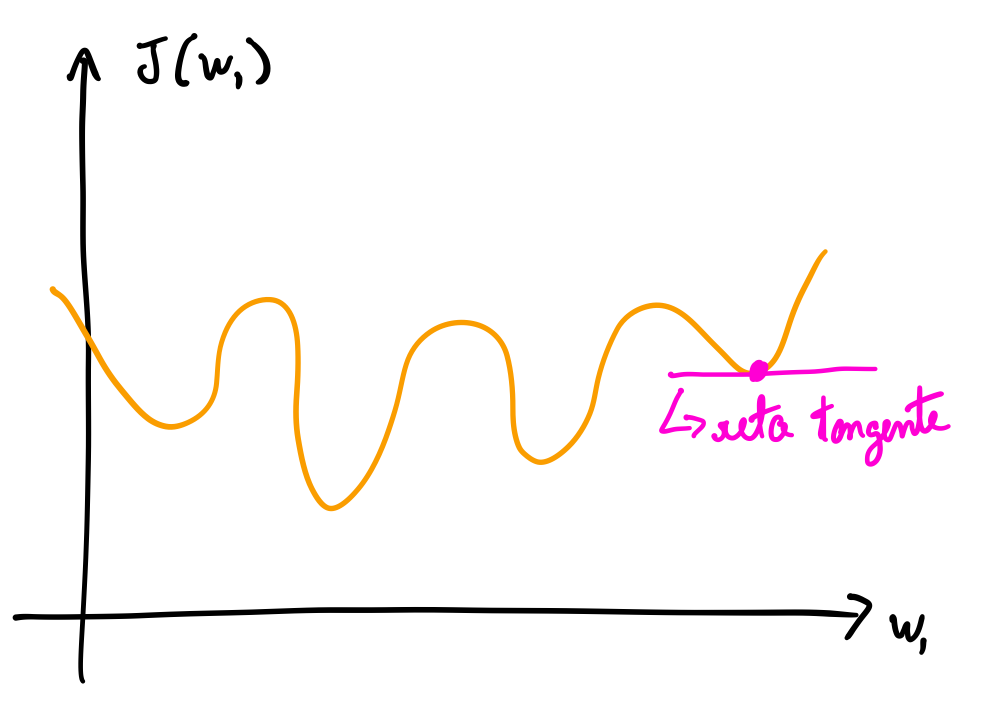
\includegraphics[scale=0.157]{./figs/Regressao_Linear_Fig22.png}
\end{minipage}%%% to prevent a space
\begin{minipage}{0.37\textwidth}
\scriptsize
\begin{equation}\nonumber
\begin{split}
w_1^{(t+1)} &= w_1^{(t)}-\alpha\frac{\partial J(\boldsymbol{w})}{\partial w_j}\\
&= w_1^{(t)}-\alpha.0\\
&= w_1^{(t)}\\
\end{split}
\end{equation}
\null
\par\xdef\tpd{\the\prevdepth}
\end{minipage}
}

\Sli{
À medida que aproximamos do ponto ótimo, o próprio gradiente descendente vai tomando passos menores, pois o termo derivativo $\frac{\partial J(\boldsymbol{w})}{\partial w_j}\rightarrow 0$.

\begin{center}
	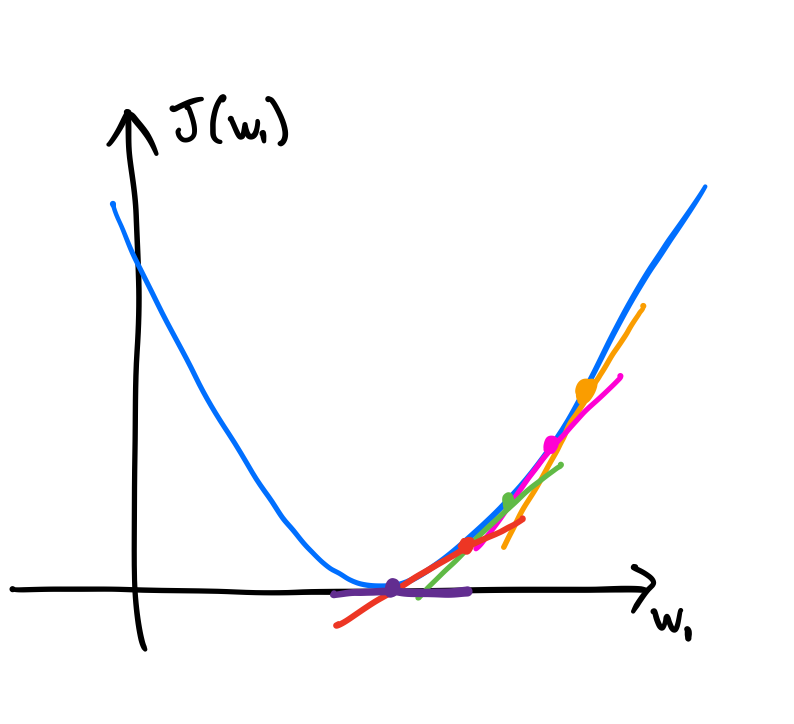
\includegraphics[scale=0.2]{./figs/Regressao_Linear_Fig23.png}
\end{center}
}

\Sli{
Precisamos, agora, calcular as derivadas parciais para $\frac{\partial J(\boldsymbol{w})}{\partial w_j}$. Temos que:
\begin{equation}
	\frac{\partial J(\boldsymbol{w})}{\partial w_0} = \frac{1}{m}\sum_{i=1}^m(h_{\boldsymbol{w}}(x_i)-y_i),
\end{equation}
e
\begin{equation}
	\frac{\partial J(\boldsymbol{w})}{\partial w_1} = \frac{1}{m}\sum_{i=1}^m[(h_{\boldsymbol{w}}(x_i)-y_i)x_i].
\end{equation}
}

\Sli{
Desta forma, o algoritmo do gradiente descendente pode ser sumarizado da seguinte forma:

\begin{enumerate}
	\item Atribua valores aleatórios para $\boldsymbol{w} = [w_0\ w_1]$.
	\item Avalie a função de custo $J(\boldsymbol{w})$.
	\item  Caso o \textbf{critério de parada tenha sido atingido}, vá para o passo 7.
	\item $w_0^{(t+1)} = w_0^{(t)}-\alpha\frac{1}{m}\sum_{i=1}^m(h_{\boldsymbol{w}}(x_i)-y_i)$.
	\item $w_1^{(t+1)} = w_1^{(t)}-\alpha\frac{1}{m}\sum_{i=1}^m[(h_{\boldsymbol{w}}(x_i)-y_i)x_i]$.
	\item Retorne ao Passo 2.
	\item Fim do algoritmo.
\end{enumerate}
Note que $w_0$ e $w_1$ precisam ser atualizados sumultaneamente!
}

\Sli{
Quais são bons critérios de parada? Podemos utilizar um número fixo de iterações ou verificar quando o valor função de custo não é mais atualizado (erro não diminui).

\begin{center}
	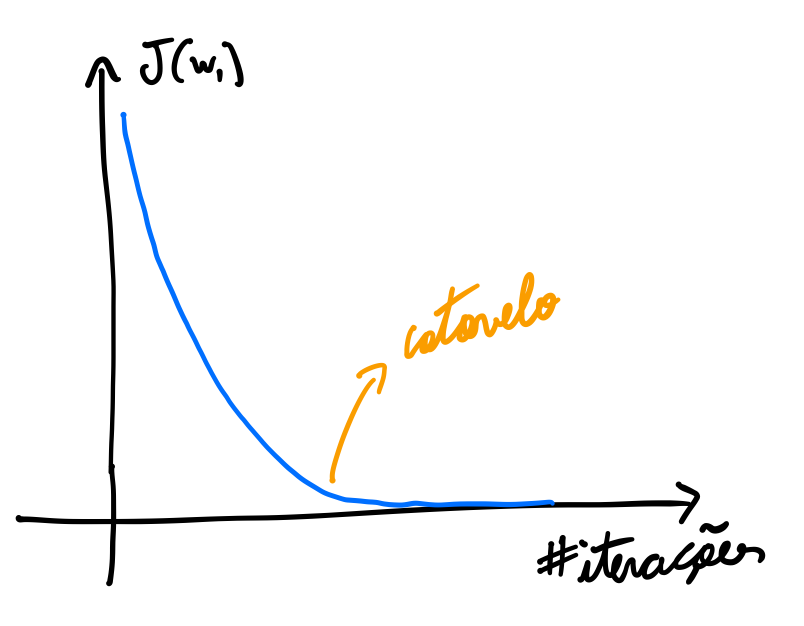
\includegraphics[scale=0.2]{./figs/Regressao_Linear_Fig24.png}
\end{center}
}

\Sli{
\secx{Regressão Linear Multivariada}\newline
\justify Suponha, agora, que tenhamos mais variáveis para representar o problema, visto que utilizar apenas o tamanho da casa não é suficiente para estimarmos o seu valor (número de quartos, capacidade da garagem, piscina, etc).\newline

\justify Neste caso, assuma que $n$ corresponde ao número dessas variáveis, ou seja, temos agora que $\boldsymbol{x}_i\in\mathbb{R}^n$. Assim sendo, nossa função hipótese possui a seguinte formulação:

\begin{align}
	h_{\boldsymbol{w}}(\boldsymbol{x})&=w_0+w_1x_1+w_2x_2+\ldots w_nx_n\\
	&=w_0+\sum_{j=1}^nw_jx^j.
\end{align}
} 

\Sli{
Para fins de simplicidade, vamos assumir que $x^0=1$, ou seja, $\boldsymbol{x}=[x^0\ x^1\ x^2\ \ldots\ x^n]\in\mathbb{R}^{n+1}$. Assim sendo, a Equação 11 pode ser escrita da seguinte forma:

\begin{align}
	h_{\boldsymbol{w}}(\boldsymbol{x}) &= w_0x^0+\sum_{j=1}^nw_jx^j\\
	&= \boldsymbol{w}^T\boldsymbol{x}.
\end{align}
A equação acima é, na verdade, a equação do hiperplano, ou seja, uma reta multimensional. Desta forma, a regressão linear multivariada generaliza a regressão linear univariada para um número maior de dimensões.
}

\Sli{
Nosso problema agora passa a ter os seguintes itens:

\begin{itemize}
	\item Função hipótese: $h_{\boldsymbol{w}}(\boldsymbol{x})=\boldsymbol{w}^T\boldsymbol{x}$.
	\item Função de custo: $J(\boldsymbol{w})=\frac{1}{2m}\sum_{i=1}^m(h_{\boldsymbol{w}}(\boldsymbol{x}_i)-y_1)^2$.
	\item Derivada parcial: $\frac{\partial J(\boldsymbol{w})}{\partial w_j}= \frac{1}{m}\sum_{i=1}^m[(h_{\boldsymbol{w}}(x_i)-y_i)x^j]$.
\end{itemize}
O algoritmo do gradiente descendente é o mesmo do apresentado para a regressão linear univariada.
}

\Sli{
Como podemos melhorar a convergência durante o aprendizado? Algumas opções:

\begin{itemize}
	\item Gradiente descendente em lotes (\emph{mini-batches}) ou \emph{online}.
	\item Gradiente descendente estocástico:
	\begin{itemize}
		\item Bom para grandes conjuntos de dados.
		\item Converge mais rápido do que o gradiente descendente (pode não avaliar todo o espaço de busca).
		\item Parecido com o gradiente descendente \emph{online}, porém é aplicado sobre amostragens aleatórias do conjunto de treinamento.
	\end{itemize}
\end{itemize}
}

\end{document}